\chapter{McCarthy-Funktion}

\section*{Lösung}

\begin{itemize}
    \item für $1 \leq i \leq 100$ liefert die Funktion den Wert $f(i) = 91$
    \item für $n > 100$ liefert die Funktion den Wert $f(n) = (n - 10)$
    \item die maximale Rekursionstiefe von $19$ tritt bei $n = 1$ auf
\end{itemize}


\section*{Anmerkungen und Ergänzungen}

Die \textit{Rekursionstiefe} ist i.A. nicht mit der Anzahl der Methodenaufrufe gleichzusetzen, worauf das Skript (Teil 2) auf Seite 34 hinweist.
\\

Die \textbf{Tiefe} eines Knotens ist im Skript auf Seite 101 beschrieben, für sie gilt

\begin{equation}
    T(n) = \begin{cases}
               0\ falls\ n\ Wurzel \\
               1\ +\ T(n')\ sonst\ (mit\ n'\ =\ Elterknoten)
    \end{cases}
\end{equation}\\

Die maximale Rekursionstiefe kann für die \code{McCarthy 91}-Methode programmatisch wie folgt ermittelt werden (s. Listing~\ref{lst:mccarthy}):

\begin{lstlisting}[language=java,caption={Ermittlung der Rekursiontiefe für die McCarthy 91-Funktion. Die Rekursionstiefe wird in einer statischen Variable gespeichert.},label=lst:mccarthy]

private static m91depth = 0;

public static int m(int n) {
    return f(n, 0);
}

private static int m(int n, int depth) {

    m91depth = Math.max(m91depth, depth);

    if (n > 100) {
        return n - 10;
    }

    return m(
        m(n + 11, depth + 1),
        depth + 1
    );

 }

\end{lstlisting}

Abbildung~\ref{fig:recursiontree} zeigt den Aufrufbaum für $n=97$:

\begin{figure}[h]
    \centering
    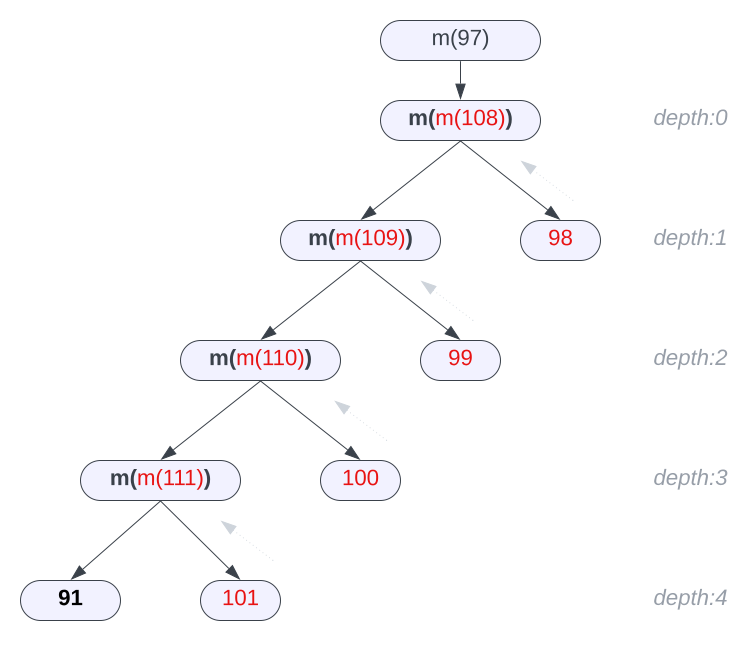
\includegraphics[
        width=12cm,
        keepaspectratio,
    ]{chapters/5. McCarthy-Funktion/img/recursiontree}
    \caption{Der Aufrufbaum für $m(97)$: Rechte Knoten werden als Rückgabewert der inneren Aufrufe an die äußeren Methoden der Vorgängerknoten übergeben, aus denen die Methodenaufrufe in den linken Teilbäumen resultieren.}
    \label{fig:recursiontree}
\end{figure}
